\documentclass[10pt, a4paper]{scrartcl}
% Packages
\usepackage[margin=1.25in]{geometry}
\usepackage{index}
\makeindex
\usepackage[utf8]{inputenc}
\usepackage[T1]{fontenc}
\usepackage{tcolorbox}
\tcbuselibrary{theorems}
\tcbuselibrary{skins}
\tcbuselibrary{breakable}
\usepackage{varwidth}
\usepackage{textcomp}
\usepackage{amsmath, amssymb}
\usepackage{esint}
\usepackage{titlesec}
\usepackage{xcolor}
\usepackage{titling}
\usepackage[linktocpage]{hyperref}
\usepackage{pgfplots}
\usepackage{multicol}
\setlength{\columnsep}{2em}
\usepackage{caption}
\usepackage{amsthm}
\usepackage{import}
\usepackage{cancel}
\usepackage{caption}
\usepackage{nicematrix}
\usepackage{mathrsfs}
\usepackage{mathtools}
%\usepackage{parskip}
\usepackage{pythonhighlight}
\usepackage{enumerate}
\usepackage{graphicx}
\usepackage{tikz}
\usepackage[italian]{babel}
\usepackage{setspace}
\setstretch{1.1}

% Titles 
\title{Note di Analisi 2}
\author{Manuel Deodato}
\date{}


% svolgimento
\newenvironment{svolgimento}{\renewcommand\qedsymbol{$\blacksquare$}\begin{proof}[Svolgimento]}{\end{proof}}


%%%%% tcolorbox setup

% Teorema e proposizione
\newtcbtheorem[number within=section]{teorema}{Teorema}
{breakable, top=0.2mm, bottom=0.2mm, boxrule=0mm,arc =.5 mm, colframe=blue!10, coltitle=black, fonttitle=\bfseries, colback=blue!5!white, theorem style=plain apart}{th}

\newtcbtheorem[number within=section]{prop}{Proposizione}
{breakable, top=0.2mm, bottom=0.2mm, boxrule=0mm,arc =.5 mm, colframe=blue!10, coltitle=black, fonttitle=\bfseries, colback=blue!5!white, theorem style=plain apart}{prop}





% Definizione
\definecolor{greendef}{HTML}{b8d8be}

\newtcbtheorem[number within=section]{definizione}{Definizione}
{breakable, top=0.2mm, bottom=0.2mm, boxrule=0mm, arc=.5mm, colframe=greendef, coltitle=black, fonttitle=\bfseries, theorem style = plain apart, colback=greendef!50!white}{def}


% Esempio
\theoremstyle{definition}
\newtheorem{esempio}{Esempio}

%\definecolor{empurple}{HTML}{6e5e89}

%\newtcbtheorem{esempio}{Esempio}{left=0mm,arc=0mm, colframe=empurple!10!white, coltitle=black, fonttitle=\bfseries, theorem style = plain, colback=empurple!20!white, colframe=empurple!90!white, boxrule=1pt, sharp corners, top=.2mm,bottom=.2mm}{es}

\tcolorboxenvironment{esempio}{blanker,breakable,left=5mm,before skip=10pt,after skip=10pt, borderline west={1mm}{0pt}{greendef}}

\numberwithin{esempio}{section}


% Lemma e Corollario
\definecolor{lemcor}{HTML}{a78d8a}

\newtcbtheorem[number within=section]{lemma}{Lemma}{breakable, top=0.2mm, bottom=0.2mm, boxrule=0mm,left=0mm,arc=.5mm, colframe=lemcor!10!white, coltitle=black, fonttitle=\bfseries, theorem style = plain apart, colframe=lemcor!50!white,colback=lemcor!20!white}{lem}
\newtcbtheorem[number within=section]{corollario}{Corollario}{breakable, top=0.2mm, bottom=0.2mm, boxrule=0mm,left=0mm,arc=.5mm, colframe=lemcor!10!white, coltitle=black, fonttitle=\bfseries, theorem style = plain apart, colframe=lemcor!50!white,colback=lemcor!20!white}{cor}



% Osservazione
\theoremstyle{definition}
\newtheorem{obs}{Osservazione}

\definecolor{coloros}{HTML}{6e5e89}

\tcolorboxenvironment{obs}{blanker,breakable,left=5mm,before skip=10pt,after skip=10pt, borderline west={1mm}{0pt}{coloros}}

\numberwithin{obs}{section}

% Nota
\newtheorem{nota}{Nota}

\definecolor{ncol}{HTML}{f9ebbe}

\tcolorboxenvironment{nota}{blanker,breakable,left=5mm,before skip=10pt,after skip=10pt, borderline west={1mm}{0pt}{ncol}}

\numberwithin{nota}{section}



%%%%%%%%%% Medie con integrali multipli
\def\Yint#1{\mathchoice
    {\YYint\displaystyle\textstyle{#1}}%
    {\YYint\textstyle\scriptstyle{#1}}%
    {\YYint\scriptstyle\scriptscriptstyle{#1}}%
    {\YYint\scriptscriptstyle\scriptscriptstyle{#1}}%
      \!\iint}
\def\YYint#1#2#3{{\setbox0=\hbox{$#1{#2#3}{\iint}$}
    \vcenter{\hbox{$#2#3$}}\kern-.51\wd0}}
\def\longdash{{-}\mkern-3.5mu{-}} 
   % consider using "\mkern-7.5mu" if esint package is loaded
\def\tiltlongdash{\rotatebox[origin=c]{15}{$\longdash$}}
\def\fiint{\Yint\tiltlongdash}

\def\Zint#1{\mathchoice
    {\YYint\displaystyle\textstyle{#1}}%
    {\YYint\textstyle\scriptstyle{#1}}%
    {\YYint\scriptstyle\scriptscriptstyle{#1}}%
    {\YYint\scriptscriptstyle\scriptscriptstyle{#1}}%
      \!\iiint}
      \def\tilongdash{\mkern6mu{-}\mkern-4mu{-}\mkern-5mu{-}} 
   % consider using "\mkern-7.5mu" if esint package is loaded
\def\titiltlongdash{\rotatebox[origin=c]{15}{$\tilongdash$}}
\def\fiiint{\Zint\titiltlongdash}

%Captions
\captionsetup[figure]{font=footnotesize,labelfont=footnotesize}
\captionsetup[table]{font=footnotesize,labelfont=footnotesize}
%Titlesec
\titleformat{\section}
{\fontsize{15}{20}\sffamily\scshape}
{\normalfont\color{gray}{\fontsize{20}{20}\selectfont\thesection}}
{0.7em}
{}
\hypersetup{colorlinks,breaklinks, linkcolor=[RGB]{74, 122, 164}}
\definecolor{asdf}{HTML}{4a7aa4}
% Personalizza la formattazione della subsection
\titleformat{\subsection}[block]{\fontsize{12}{20}\bfseries}{\normalfont\thesubsection}{.5em}{}


% Personalizza la formattazione della subsubsection
\titleformat{\subsubsection}[block]{\fontsize{10}{20}\bfseries}{\normalfont\thesubsubsection}{.5em}{}

% Maketitle customization
\renewcommand{\maketitle}{
\begin{center}
{\sffamily
{\fontsize{20}{20}\selectfont\MakeUppercase\thetitle}}

\vspace{0.2in}

{\large\scshape\sffamily\theauthor}
\end{center}
}

%Evaluate symbol
\DeclareMathOperator{\di}{d\!}
\newcommand*\Eval[3]{\left.#1\right\rvert_{#2}^{#3}}

%%%%%%% Numero delle equazioni in formato a.b
\numberwithin{equation}{subsection}
%%%%%

%%%%%%%%%% Personalizzazione numeri lista
\renewcommand{\theenumi}{(\arabic{enumi})}

%%%% Table of contents

\usepackage[titles]{tocloft}

\renewcommand{\cftdot}{}
\usepackage{titletoc}
%\setcounter{tocdepth}{2}

%%%%%%%%%%%%%%%% Toc style

% Personalizzazione scritta indice


% Font
% \usepackage[osf]{newpxtext}
\usepackage{sansiwona}


\begin{document}
\maketitle
\vspace{9cm}
\begin{figure}[h!]
	\centering
	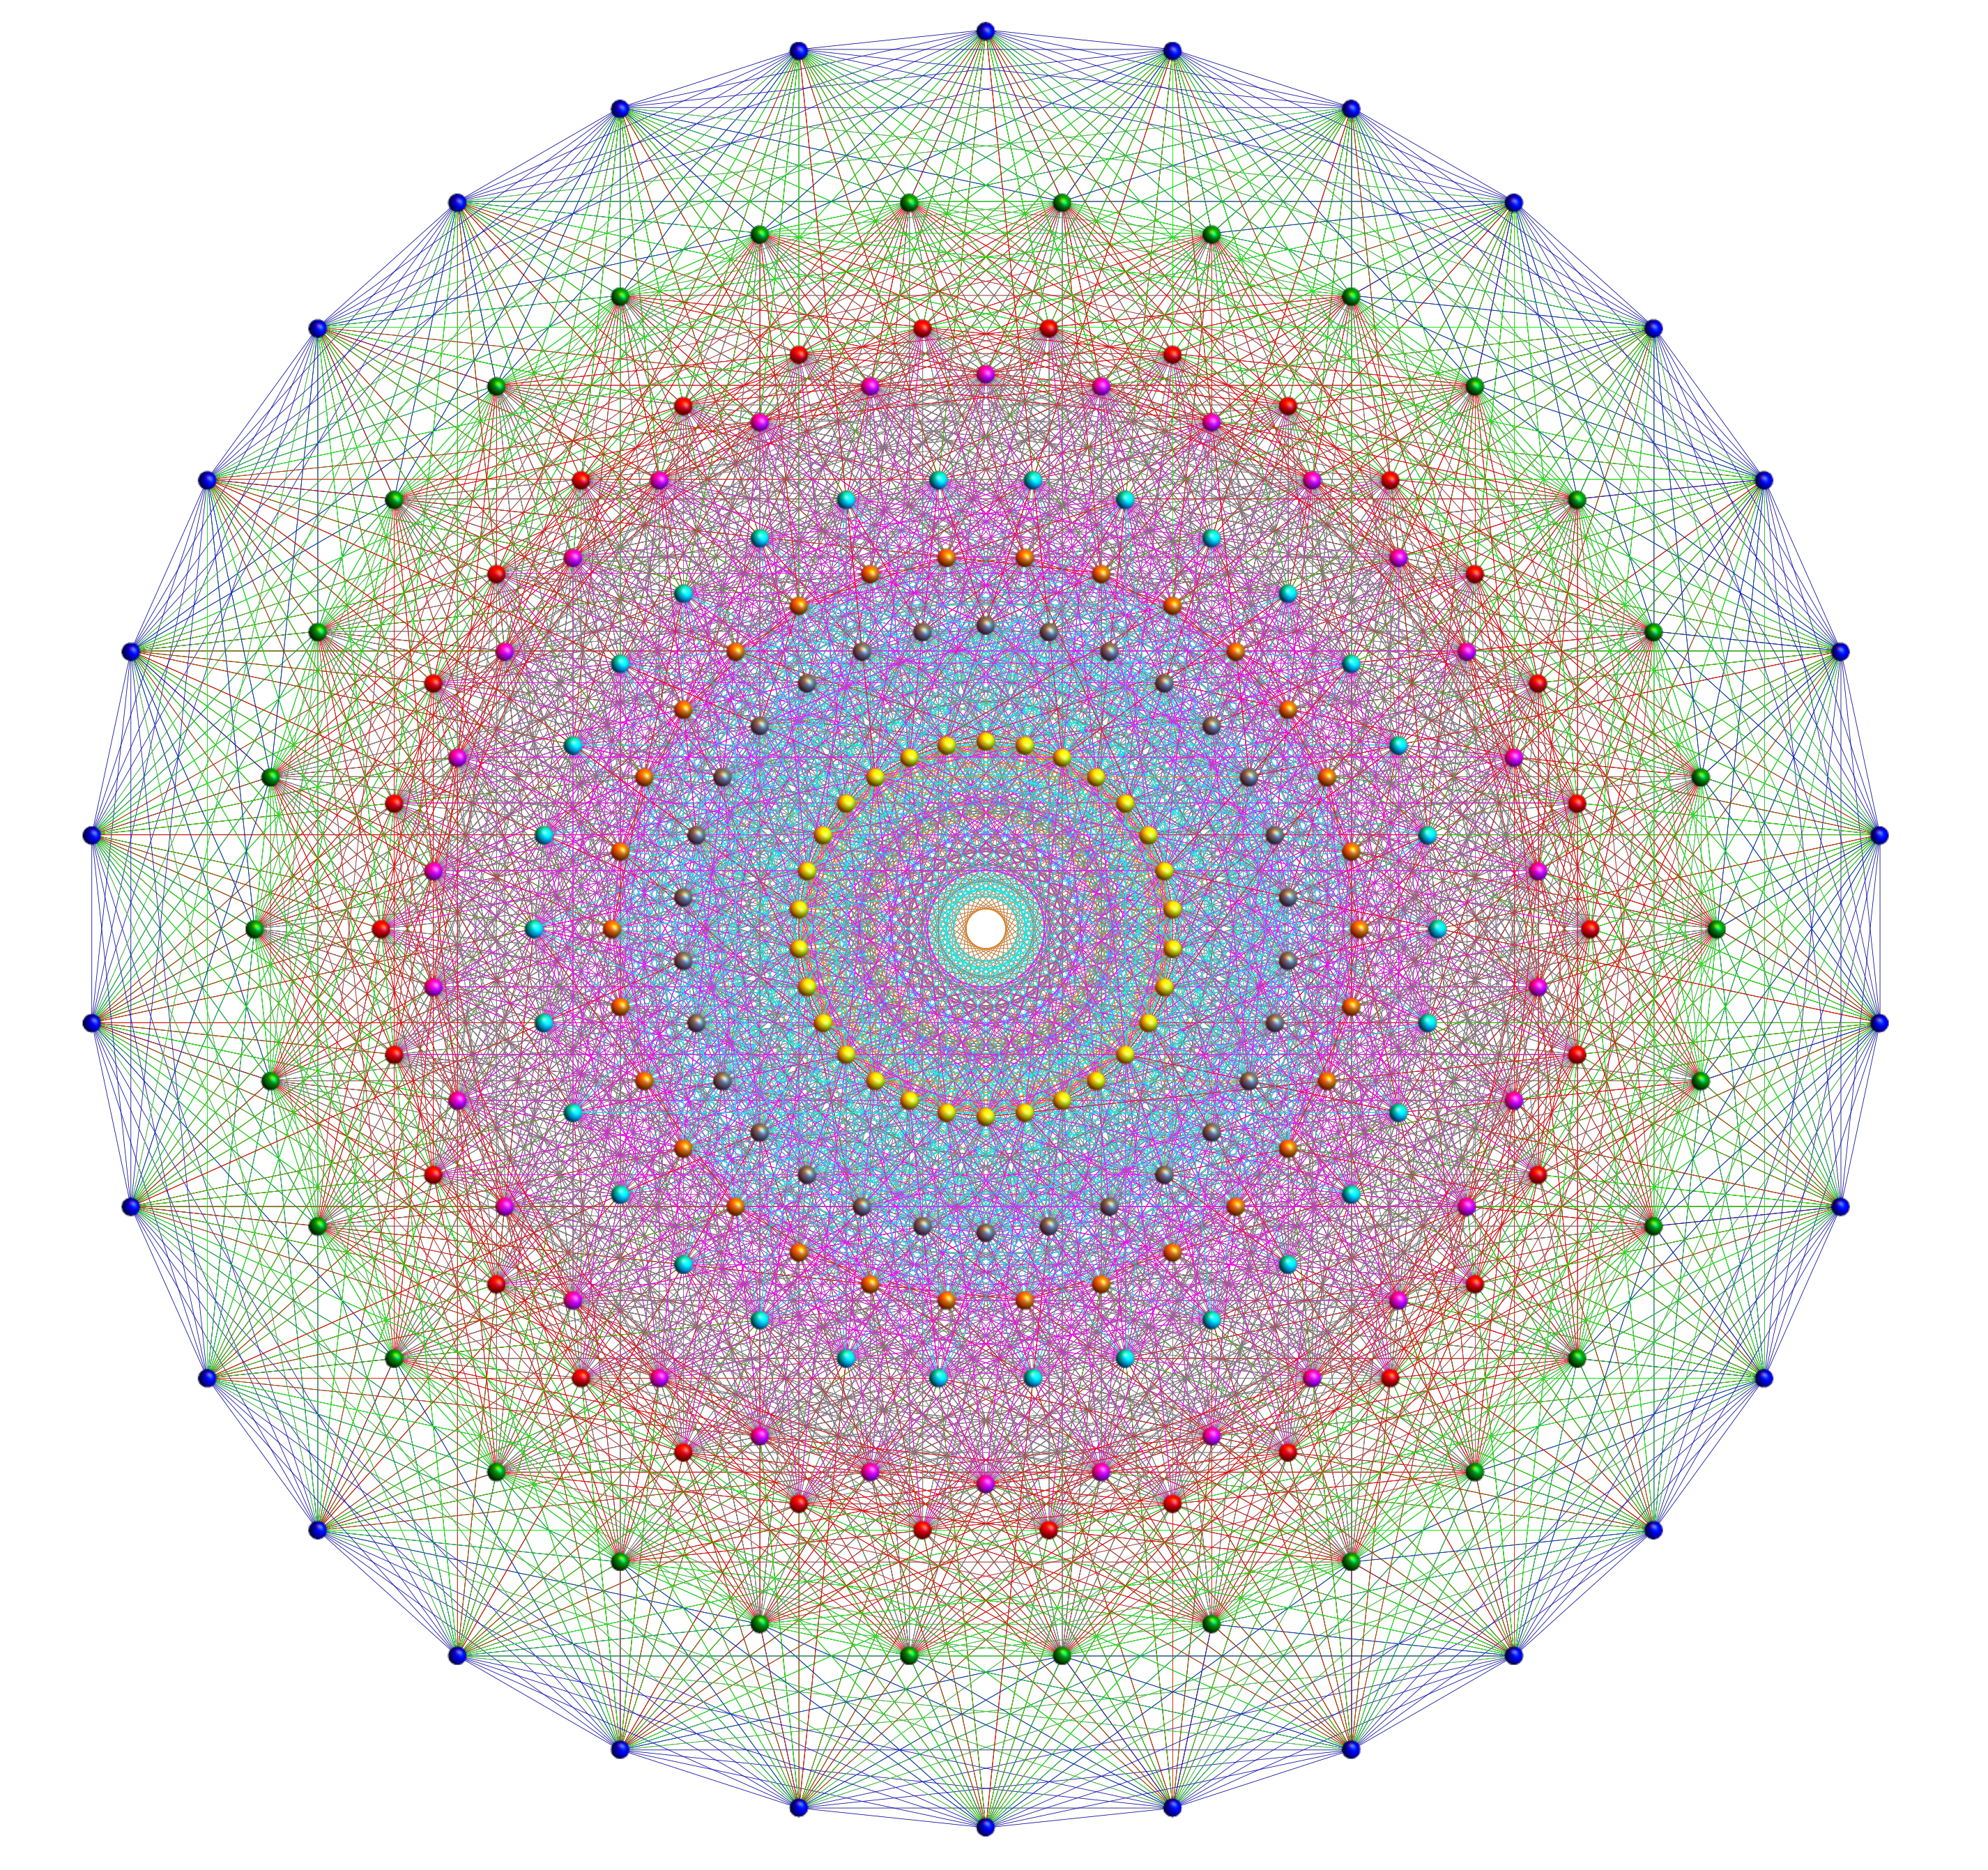
\includegraphics[width=1\columnwidth]{front.png}
\end{figure}
\newpage
\tableofcontents 
\newpage
\section{Calcolo differenziale in pi\`u variabili}
\subsection{Derivate parziali}

Una funzione di pi\`u variabili $f(x,y):\mathbb{R}^2 \to \mathbb{R}$ pu\`o essere derivata mantenendo fissa una variabile e derivando rispetto all'altra. Questo corrisponde al valutare la variazione di $f$ lungo un asse specifico.
\begin{definizione}
	{Derivata parziale}{}
	Sia $f(x_1,\ldots,x_n) :\mathbb{R}^n \to \mathbb{R}$; la sua derivata parziale rispetto a $x_k$ \`e:
	\begin{equation}
		\frac{\partial f}{\partial x_k}(x_1,\ldots,x_n) = \lim_{h \to 0} \frac{f(x_1,\ldots,x_k + h, \ldots, x_n)-f(x_1,\ldots,x_k,\ldots,x_n)}{h}
	\end{equation}
\end{definizione}
\noindent Il vettore che ha per componenti le derivate di $f$ rispetto a ciascuna delle sue variabili si chiama \textbf{gradiente} e si indica con $\nabla f$.

\subsection{Derivate direzionali}

\`E possibile studiare la variazione di $f$ lungo una particolare direzione individuata dal versore $\hat{n}$. Una retta parallela a $\hat{n}$ e passante per un punto $x$ si individua con $x+t \hat{n}$; fissando i punti $x$ e $\hat{n}$, $g(t) := f(x+t\hat{n})$ \`e una funzione di una variabile e $g'(0)$ \`e la derivata direzionale di $f$ lungo $\hat{n}$:
\begin{equation}
	\frac{\partial f}{\partial \hat{n}} (x) = g'(0) = \lim_{h \to 0} \frac{f(x+h\hat{n}) - f(x)}{h}
\end{equation}
Pi\`u in generale:
\begin{equation}
	g'(t) \overset{\text{def}}{=} \lim_{h \to 0} \frac{g(t+h) - g(t)}{h} = \lim_{h \to 0} \frac{f(x_t+ h \hat{n}) - f(x_t)}{h} \equiv \frac{\partial f}{\partial \hat{n}} (x_t)
\end{equation}
con $x_t = x+t \hat{n}$. 
\begin{obs}
	Conoscendo $\nabla f$, si pu\`o calcolare la derivata direzionale di $f$ come $\nabla f \cdot \hat{n}$.
\end{obs}
\begin{esempio}
	Si calcola la derivata direzionale di $f(x,y) = x^2 y - e^{x+y} $ lungo la direzione $\hat{n} = \left(\frac{1}{2}, \frac{\sqrt{3} }{2}\right) $.
	\begin{svolgimento}
		Si ha 
		\[
		g(t) = f\left(x + \frac{t}{2}, y + \frac{\sqrt{3} }{2}t\right) = \left(x + \frac{t}{2}\right) ^2 \left(y + \frac{\sqrt{3} }{2}t\right) - \exp \left[ x + y + t\left(\frac{1}{2} + \frac{\sqrt{3} }{2}\right)  \right] 
		\] 
		Allora 
		\[
		\frac{\partial f}{\partial \hat{n}} (x,y) = g'(0) = xy + \frac{\sqrt{3} }{2}x^2 - \left(\frac{1}{2}+ \frac{\sqrt{3} }{2} \right) e^{x+y} 
		\] 
		Alternativamente $\nabla f = \left(2xy - e^{x+y} , x^2 - e^{x+y} \right) $, quindi $\partial _{\hat{n}} f = \nabla f \cdot \hat{n} =xy - \frac{1}{2} e^{x+y} +\frac{\sqrt{3} }{2} x^2 - \frac{\sqrt{3} }{2}e^{x+y} = xy + \frac{\sqrt{3} }{2}x^2 - \left(\frac{1}{2}+\frac{\sqrt{3} }{2}\right) e^{x+y}   $.
	\end{svolgimento}
\end{esempio}
\begin{teorema}
	{}{}
	Se $f:A\subset \mathbb{R}^2 \to  \mathbb{R}$ ha un massimo o minimo relativo in $x_0$ interno ad $A$ e se ammette derivata lungo $\hat{n}$ in $x_0$, allora:
	\begin{equation}
		\frac{\partial f}{\partial \hat{n}} (x_0)= 0 
	\end{equation}
	\begin{proof}
		Si prende $g(t) = f(x_0 + t \hat{n})$ che, per costruzione, ha un minimo in $t=0$, quindi $g'(0) = 0$, da cui segue la tesi.
	\end{proof}
\end{teorema}
\noindent In particolare, se $f$ \`e derivabile in $x_0$, tutte le derivate parziali si annullano in quel punto; in questo caso, $x_0$ \`e detto \textbf{punto stazionario}.

\begin{obs}
	Nel caso a una variabile, i punti di massimo/minimo che cadevano sulla frontiera di un insieme erano, solitamente, un numero finito; qua chiaramente non \`e pi\`u cos\`i.
\end{obs}
\begin{esempio}
	Calcolare massimi e minimi di $f(x,y) = (x^2 + y^2 - 1)e^{x+y} $ nel cerchio chiuso centrato nell'origine e di raggio $1$.
	\begin{svolgimento}
		Sul bordo del cerchio $x^2 + y^2 = 1$, quindi $f\equiv 0$. All'interno:
		\[
			\begin{split}
				&f_x = 2x e^{x+y}  + (x^2 + y^2 -1)e^{x+y} \\
				&f_y = 2y e^{x+y} + (x^2 + y^2 - 1) e^{x+y} 
			\end{split}
		\] 
	che si annullano quando 
	\[
	\begin{split}
		&x^2 + y^2 + 2x - 1 = 0\\
		&x^2 + y^2 + 2y - 1 = 0
	\end{split}\Rightarrow 2x - 2y = 0 \Rightarrow x=y
	\] 
Sostituendo $x=y$ nella prima equazione, ad esempio, si ottengono due soluzioni, una sola delle quali appartiene al cerchio; questo corrisponder\`a al punto di minimo della funzione:
\[
f\left(\frac{\sqrt{3} -1}{2}, \frac{\sqrt{3} -1}{2}\right) = (1-\sqrt{3} ) e^{\sqrt{3} -1}  < 0
\] 
\end{svolgimento}
\end{esempio}
\noindent In pi\`u dimensioni vale un analogo del teorema di Lagrange:
\begin{teorema}
	{}{}
	Sia $f(x) : A \subset \mathbb{R}^n \to \mathbb{R}$ e $x_0 \in A$, con $I(x_0,r) \subset A$. Considerando una direzione $\hat{n}$, si definisce $g(s) = f(x_0+ s \hat{n})$ per $\lvert s \rvert <r$. Vale l'analogo del teorema di Lagrange:
	\begin{equation}
		f(x_0+s\hat{n}) - f(x_0) = g(s) - g(0) = s g'(\tau ) = s \frac{\partial f}{\partial \hat{n}} (x_0 + \tau \hat{n})
	\end{equation}
\end{teorema}

\subsection{Derivate successive}

Sia $f$ una funzione per cui esistono le derivate prime e sono anch'esse derivabili; le derivate seconde potranno essere derivate prima rispetto a $x_i$ e poi rispetto a $x_j$ o viceversa. In generale se $f$ \`e una funzione di $m$, si hanno $m^n$ derivate di ordine $n$. Per le derivate seconde miste\footnote{Chiaramente il risultato vale in generale, ma si affronta per funzione di due variabili nel caso delle derivate seconde miste per semplicit\`a.} vale il seguente.
\begin{teorema}
	{Teorema di Schwarz}{}
	Sia $f$ una funzione derivabile in un intervallo $I$ del punto $(x,y)$ e siano queste continue nello stesso intervallo; allora $f_{xy} (x,y) = f_{yx} (x,y)$.
	\begin{proof}
		Siano $h,k \in \mathbb{R}:(x+h,y+k) \in I$ e sia
		\[
		A(h,k) = f(x+h,y+k) - f(x+h,y) - f(x,y+k) + f(x,y)
		\] 
		Prendendo $p(t) = f(t,y+k) - f(t,y)$, si ha $A(h,k) = p(x+h) - p(x)$; per Lagrange:
		\[
			A(h,k) = p'(\xi ) h = \big[f_x(\xi ,y+k) - f_x(\xi ,y)\big]h ,\ x< \xi <x+h
		\] 
		Applicando nuovamente Lagrange, si ha $A(h,k) = f_{yx} (\xi, \eta) hk, \ y<\eta < y+k$. Ripetendo il discorso con $q(t) = f(x+h,t) - f(x,t)$, si trova $A(h,k) = f_{xy} (\sigma ,\tau ) hk$, quindi $f_{yx}(\xi ,\eta) =f_{xy} (\sigma ,\tau ) $, dove $x<\sigma <x+h$ e $y<\tau <y+k$. Prendendo il limite per $h,k\to 0$, risulta $f_{xy} (x,y) = f_{yx} (x,y)$ per continuit\`a delle derivate seconde.
		
	\end{proof}
\end{teorema}
\noindent Come per funzioni di una variabile, vale la formula di Taylor.
\begin{teorema}
	{Formula di Taylor}{}
	Sia $f(x)$ di classe $C^2$ in $A \subset \mathbb{R}^n$ e $x_0$ punto interno ad $A$; in un intorno di $x_0$, allora, si ha:
	\begin{equation}
		f(x) = f(x_0) + \left\langle \nabla f(x_0), x-x_0 \right\rangle + \frac{1}{2} \left\langle Hf(x_0) (x-x_0), x-x_0 \right\rangle + R_2(x;x_0)
	\end{equation}
	con 
	\[
	\lim_{x \to x_0} \frac{R_2(x;x_0)}{\left\lVert x-x_0 \right\rVert ^2} = 0
	\] 
	
\end{teorema}

\subsection{Funzioni differenziabili}


Una funzione derivabile, anche in ogni direzione, non \`e necessariamente continua in pi\`u variabili.
\begin{esempio}
	La funzione $f(x,y) = \begin{cases}
		\frac{xy^2}{x^2 + y^2}& , \ (x,y)\neq 0\\
		0 & , \ (x,y) =0 
	\end{cases}$ ha derivate in ogni direzione nel punto $(0,0)$, ma non \`e continua; prendendo $x_k = (1 / k , 1/k^2)$ per $k\to \infty$, si ha $x_k\to (0,0)$, ma $f(x_k) = \frac{1/k^4}{2 / k^4} \to \frac{1}{2}$.
\end{esempio}

\begin{definizione}{Differenziabilit\`a}{}
	Una funzione $f(x)$ si dice differenziabile in $x_0$ se \`e derivabile in $x_0 $ e se:
	\begin{equation}
		\lim_{x \to x_0} \frac{f(x) - f(x_0) - \langle \nabla f(x_0) , x -x_0 \rangle}{\left\lVert x - x_0 \right\rVert } = 0
	\end{equation}
\end{definizione}
\noindent Questa definizione impone che una funzione sia differenziabile in punto se esiste un piano tangente che la approssima precisamente nel punto stesso.

\begin{teorema}
	{}{}
	Una funzione $f(x)$ differenziabile in $x_0$ \`e continua in $x_0$ ed \`e derivabile in ogni direzione.
	\begin{proof}
		Si mostra che \`e continua:
		\[
		f(x) - f(x_0)  = \frac{f(x) - f(x_0) - \langle \nabla f(x_0) , x-x_0 \rangle}{\left\lVert x-x_0 \right\rVert } \left\lVert x-x_0 \right\rVert + \langle \nabla f(x_0) , x-x_0 \rangle
		\] 
		Per $x\to x_0$ il primo termine di destra va a $0$ per assunzione di differenziabilit\`a e l'altro anche perch\'e diventa un prodotto scalare per $0$, quindi si verifica $\lim_{x \to x_0} f(x) = f(x_0)$.

		Data generica direzione $\hat{v}$ con $x = x_0 + t \hat{v}$, usando ancora definizione di differenziabilit\`a:
		\[
		\lim_{t \to 0} \frac{f(x_0 + t \hat{v})- f(x_0) - \langle \nabla f(x_0), t \hat{v} \rangle}{t} = 0 
		\] 
Visto che $\langle \nabla f(x_0 ) , t \hat{v} \rangle = t \langle \nabla f(x_0) ,\hat{v} \rangle$, si ottiene la tesi.
	\end{proof}
\end{teorema}
\noindent La direzione di massimo incremento di una funzione \`e quella del gradiente. Per mostrarlo, si parte da $x_0$, assumendo che non sia un punto stazionario; si definisce, allora, $\hat{n} = \frac{\nabla f(x_0)}{\left\lVert \nabla f(x_0) \right\rVert} $, da cui:
\[
\frac{\partial f}{\partial \hat{n}} (x_0) = \langle \nabla f(x_0), \hat{n} \rangle = \left\lVert \nabla f(x_0) \right\rVert 
\] 
Prendendo altra direzione generica $\hat{v}$, si ha:
\[
\frac{\partial f}{\partial \hat{v}} (x_0) = \langle \nabla f(x_0) , \hat{v}  \rangle \le  \left\lVert \nabla f(x_0) \right\rVert \left\lVert \hat{v} \right\rVert = \left\lVert \nabla f(x_0) \right\rVert \equiv \frac{\partial f}{\partial \hat{n}} (x_0)
\] 
Dalla definizione di funzione differenziabile il piano $z = f(x_0,y_0) +f_x(x_0,y_0) (x-x_0) + f_y(x_0,y_0) (y-y_0)$ \`e quello che meglio approssima la funzione in $(x_0,y_0)$.

Si \`e concluso che una funzione differenziabile \`e derivabile in ogni direzione, ma una funzione derivabile non \`e differenziabile in generale. Vale, per\`o, il seguente.
\begin{teorema}
	{Teorema del differenziale totale}{}
	Sia $f(x)$ derivabile in $x_0$ e siano le sue derivate continue nello stesso punto; allora $f$ \`e differenziabile in $x_0$.
	\begin{proof}
		Si vuole dimostrare che
		\[
		\lim_{(x,y) \to (x_0,y_0)} \frac{f(x,y) - f(x_0,y_0) - f_x(x_0,y_0) (x-x_0) - f_y(x_0,y_0)(y-y_0)}{\sqrt{(x-x_0)^2 + (y-y_0)^2} } = 0
		\] 
		Si usa il teorema di Lagrange per riscrivere $f(x,y) - f(x_0,y_0)$:
		\[
		\begin{split}
			&f(x,y_0) - f(x_0,y_0) = f_x(\xi ,y_0) (x-x_0),\ x_0<\xi <x\\
			&f(x,y) - f(x,y_0) = f_y(x ,\eta) (y-y_0), \ y_0 < \eta < y\\
			&\Rightarrow f(x,y) - f(x_0,y_0) = f_x(\xi ,y_0) (x-x_0) + f_y(x,\eta) (y-y_0)
		\end{split}
		\] 
	Il limite scritto sopra si riscrive come:
	\[
		\begin{split}
			\lim_{(x,y) \to (x_0,y_0)} \big[f_x(\xi ,y_0) - f_x(x_0,y_0)\big] &\frac{x-x_0}{\sqrt{(x-x_0)^2 + (y-y_0)^2} } + \\ 
											  &+\big[f_y(x,\eta) - f_y(x_0,y_0)\big] \frac{y-y_0}{\sqrt{(x-x_0)^2 + (y-y_0)^2} }
		\end{split}
	\] 
	Essendo le frazioni $\le 1$ e visto che le quantit\`a fra parentesi quadre, questo limite si maggiora con la somma delle parentesi quadre, che tende a $0$ per $(x,y) \to (x_0,y_0)$.
	\end{proof}
\end{teorema}
\subsection{Funzioni composte}
	Data una funzione $x(t) : \mathbb{R}^k \to \mathbb{R}^n$, si definisce, per una generica direzione $v$:
	\begin{equation}
		\frac{\partial x}{\partial v} = \left(\frac{\partial x_1}{\partial v}, \ldots , \frac{\partial x_n}{\partial t}  \right) ^\top
	\end{equation}
Vale il seguente per la derivata della funzione composta.
\begin{teorema}
	{}{}
	Siano $E \subset  \mathbb{R}^k , \ F \subset \mathbb{R}^n$ e $x(t) : E \to F , \ f(x) : F \to \mathbb{R}$ funzioni di classe $C^1$. Allora la funzione composta $g(t) = f(x(t)) : E \to\mathbb{R}$ \`e di classe $C^1$ e per ogni direzione $v$:
	\begin{equation}
		\frac{\partial g}{\partial v} (t) =\left\langle \nabla f\big(x(t)\big), \frac{\partial x}{\partial v} (t) \right\rangle
	\end{equation}
	\begin{proof}
		Si ha $g(t + h v) -g(t) = f\big(x(t+hv)\big) - f\big(x(t)\big) = f\big(x(t) + [x(t+hv) - x(t)]\big) - f\big(x(t)\big)$. Si prende $s = \lVert x(t+hv) - x(t) \rVert $ e la direzione$w = \frac{x(t+hv) - x(t)}{s}$ e si usa il teorema di Lagrange:
		\[
		g(t+hv) - g(t) = f\big(x(t) + s w\big) - f\big(x(t)\big) = s \frac{\partial f}{\partial w} \big(x(t) + \tau w\big) = s \left\langle \nabla f \big(x(t) + \tau  w\big), w \right\rangle
		\] 
	con $0<\tau <s$. Dividendo per $h$ e prendendo il limite $h\to 0$, per definizione $s \to 0$ e, quindi, $\tau  \to 0$, mentre $\frac{x(t+hv) - x(t)}{h}\to \frac{\partial x}{\partial v} (t)$ quindi:
\[
\lim_{h \to 0} \frac{g(t+ hv) -g(t)}{h} = \lim_{h \to 0} \left\langle \nabla f\big(x(t) + \tau  w\big), \frac{x(t+hv) - x(t)}{h} \right\rangle = \left\langle\nabla f\big(x(t)\big), \frac{\partial x}{\partial v} (t)  \right\rangle
\] 
	\end{proof}
\end{teorema}
\noindent Nel caso particolare $k=1$, $x(t)$ \`e una curva e $g(t)$ \`e funzione di una sola variabile con
\[
g'(t) = \sum_{h=1}^{n} \frac{\partial f}{\partial x_h} \big(x(t)\big) x'_h(t) \equiv \Big\langle \nabla f \big(x(t)\big), x'(t) \Big\rangle
\] 
Spesso si prende $x(t) = x + t v $, cio\`e retta passante per $x$ lungo direzione $v$; in questo caso $g'(t) = \nabla f(x+tv) \cdot  v$. Se le derivate seconde sono continue, le derivate prime sono differenziabili e si pu\`o scrivere:
\begin{equation}
	g''(t)	= \sum_{i=1}^{n} v_i \frac{d }{d t} D_i f (x+tv) = \sum_{i=1}^{n} v_i \sum_{j=1}^{n} v_j D_{ij} f(x+tv)
\end{equation}
Indicando con $Hf = \nabla f \nabla ^\top$ la matrice Hessiana di $f$, allora $\sum_{j}^{} v_j D_{ij} f(x+tv) \equiv \left[ Hf(x+tv) v\right]_i $, cio\`e \`e la componente $i$-esima del vettore tra parentesi quadre, essendo $Hf$ una matrice. Allora:
\begin{equation}
	\begin{split}
		&g'(0) = \nabla f(x) \cdot v \\ 
		& g''(0) = \langle Hf(x) v , v \rangle
	\end{split}
\end{equation}
 
\subsection{Massimi e minimi relativi}

Perch\'e una funzione $f$ di pi\`u variabili abbia un punto di massimo o di minimo in $x_0$, \`e condizione necessaria che per ogni direzione $v$, valga $g'(0) = 0$ e $g''(0) \le 0$ o $g''(0) \ge 0$, cio\`e:
\begin{equation}
	\begin{split}
		&\langle Hf (x_0) v , v \rangle \le 0 \text{ punto di massimo}\\
		&\langle Hf (x_0) v , v \rangle \ge 0 \text{ punto di minimo}
	\end{split}
\end{equation}
Allora vale il seguente.
\begin{teorema}
	{}{}
	Sia $f(x)$ una funzione con derivate seconde continue; se in $x_0$, $\nabla f (x_0) = 0$ e la matrice Hessiana \`e tale che $Hf(x_0) > 0$ (definita positiva), allora $x_0$ \`e di minimo relativo per $f$. Se fosse $Hf(x_0) < 0$, $x_0$ sarebbe di massimo relativo.
\end{teorema}
\noindent Possono verificarsi altri due casi:
\begin{itemize}
	\item se $\langle H f(x_0)v ,v \rangle $ assume sia valori positivi che negativi al variare di $v$, si ha un \textbf{punto di sella};
	\item se la matrice Hessiana \`e semidefinita, ma non definita, non si pu\`o concludere niente e bisogna esaminare cosa accade attorno a $x_0$.
\end{itemize}

\newpage 

\section{Calcolo integrale in pi\`u variabili}

\subsection{Integrazione in dimensioni superiori}
Per le definizioni di base, si deve definire cos'\`e un rettangolo.
\begin{definizione}
	{}{}
	Dati due intervalli $[a.b)$ e $[c,d)$, il rettangolo che identificano \`e definito come $R = [a,b) \times  [c,d)$, con $a\le x< b$ e $c\le y<d$.
\end{definizione}
\noindent Si suddividono due intervalli in intervalli pi\`u piccoli, cio\`e $[a,b)$ si suddivide in $n$ sotto-intervalli $I_h = [x_{h-1} ,x_h)$, con $x_0 =a , \ldots x_n = b$ e $[c,d)$ in $m$ sotto-intervalli $J_k = [y_{k-1} ,y_k)$. Allora il rettangolo sar\`a suddiviso in $n\times m$ sotto-rettangoli $R_{hk}  = I_h \times J_k$.

Una funzione semplice $\varphi (x)$ \`e una funzione che assume un valore costante su ogni sotto-rettangolo e che vale $0$ fuori da $R$. Indicando con $\lambda _{hk}$ il valore costante che assume in $R_{hk} $:
\begin{equation}
	\varphi (x)= \sum_{h=1}^{n} \sum_{k=1}^{m} \lambda _{hk} \chi _{R_{hk} } (x)
\end{equation}
con $\chi _D$ funzione caratteristica del dominio $D$. L'integrale di funzioni simili \`e dato da:
\begin{equation}
	\int \varphi (x) \ dxdy = \sum_{h=1}^{n} \sum_{k=1}^{m} \lambda _{hk} m(R_{hk} )= \sum_{h=1}^{n} \sum_{k=1}^{m} \lambda _{hk} m(I_h) m(J_k) = \sum_{h=1}^{n} \sum_{k=1}^{m} \lambda _{hk} (x_h -x_{h-1} ) (y_k - y_{k-1} )
\end{equation}
\`E necessario dare anche la definizione di supporto di una funzione:
\begin{definizione}
	{}{}
	Il supporto di una funzione $f$ \`e la chiusura dell'insieme in cui $f\neq 0$, cio\`e:
	\begin{equation}
		\operatorname{supp} (f) = \overline{\left\{ x : f(x) \neq 0 \right\} }
	\end{equation}
\end{definizione}
\noindent Infine, si indica con $\mathscr{S}^+(D)$ la classe delle funzioni semplici $\varphi $ che maggiorano $f$ in $D$ e $\mathscr{S}^-(D)$ la classe delle funzioni semplici $\psi $ che minorano $f$ in $D$; da questo, si ha la seguente definizione di integrale di Riemann.
\begin{definizione}
	{Integrazione di funzioni a supporto compatto}{}
	Sia $f$ una funzione a supporto compatto, con $\operatorname{supp} (f) \subset K$; $f$ \`e integrabile secondo Riemann se:
	\begin{equation}
		\sup_{\psi \in \mathscr{S}^-(K)}  \int \psi  \ dx dy = \inf_{\varphi \in \mathscr{S}^+(K)}  \int \varphi \ dxdy
	\end{equation}
	dove
	\begin{equation}
		\begin{split}
			&\int_{*} f(x) \ dx =  \inf_{\varphi \in \mathscr{S}^+(K)}  \int \varphi \ dxdy \ \text{ integrale inferiore} \\
			&\int^{*} f(x) \ dx =  \sup_{\psi  \in \mathscr{S}^-(K)}  \int \psi  \ dxdy \ \text{ integrale superiore} \\
		\end{split}
	\end{equation}
	La condizione di integrabilit\`a si pu\`o esprimere come:
	\begin{equation}
		\int_{*} f(x) \ dx= \int^{*} f(x) \ dx
	\end{equation}
\end{definizione}
\begin{obs}
	Anche per pi\`u variabili, \`e condizione sufficiente e necessaria perch\'e $f$ a supporto compatto sia integrabile che $\forall \varepsilon >0$, esistono funzioni semplici $\varphi ,\psi $ tali che:
	\begin{equation}
		\int \varphi  \ dxdy - \int \psi  \ dxdy < \varepsilon 
	\end{equation}
\end{obs}
\subsection{Misura di insiemi}
L'integrabilit\`a di una funzione su un certo insieme $E$ \`e legata alla misura dell'insieme stesso.
\begin{definizione}
	{Misurabilit\`a di insiemi}{}
	Un insieme $E$ \`e \textit{misurabile} (secondo Peano-Jordan) se la sua funzione caratteristica $\varphi _E$ \`e integrabile. In questo caso, la misura \`e:
	\begin{equation*}
		m(E) = \int \varphi _E \ d\mathbf{x} 
	\end{equation*}
\end{definizione}
\noindent Se $\varphi _E$ \`e integrabile, allora $\forall \varepsilon >0$, si avrebbero $\psi ,\varphi $ funzioni semplici con $\psi \le  \varphi _E \le \varphi $ tali che:
\[
\int \varphi  \ d\mathbf{x}  - \int \psi \ d\mathbf{x} < \varepsilon 
\] 
L'idea \`e suddividere il piano $x,y$ in rettangoli $R_{hk} $ dove $\varphi =1$ nei rettangoli $R_{hk} $ che hanno punti in comune con $E$ ed \`e nulla negli altri, mentre si prende $\psi =1 $ nei rettangoli contenuti in $E$ e pari a $0$ negli altri. Cos\`i facendo, l'integrale di $\varphi $ \`e la somma delle misure dei rettangoli $R_{hk}$ che hanno punti in comune con $E$, mentre quello di $\psi $ \`e la somma delle misure degli $R_{hk} $ contenuti in $E$. Il risultato della differenza \`e la somma delle misure dei rettangoli che hanno punti in comune con $E$, ma che non vi sono contenuti, quindi sar\`a la somma delle misure dei rettangoli che hanno punti in comune con la frontiera di $E$.

Si definisce \textbf{plurirettangolo} l'unione $P$ di un numero finito di rettangoli senza punti comuni, la cui misura coincide con la somma delle misure dei rettangoli che lo compongono; si ha la seguente.
\begin{prop}
	{}{mis21}
	Un insieme $E$ \`e misurabile $\iff \forall \varepsilon >0, \ \exists $ un plurirettangolo $P$ contenuto in $E$ e un plurirettangolo $Q$ che contiene $E$ tali che $m(Q) - m(E) < \varepsilon $.
\end{prop}
\noindent Usando Prop \ref{prop:mis21}, se $P,Q$ plurirettangoli t.c. $P \subset E \subset Q$, con $m(Q-P) = m(Q) - m(P)$, si ha che:
\begin{center}
	\textit{Un insieme $E$ \`e misurabile $\iff \forall \varepsilon > 0$ esiste $Z$ plurirettangolo che contiene $\partial E$, con $m(Z)<\varepsilon $.} 
\end{center}
Quindi:
\begin{center}
	\textit{Un insieme $E$ \`e misurabile (secondo Peano-Jordan) $\iff$ la sua frontiera\newline $\partial E$ ha misura nulla.} 
\end{center}
\begin{prop}
	{}{}
	Se due insiemi $A,B$ sono misurabili, allora sono misurabili anche $A \cup B , \ A \cap B $ e $A \setminus B$.
	\begin{proof}
		$A,B$ misurabili $\implies$ $\partial A, \ \partial B$ sono contenute in plurirettangoli $Z_A,Z_B$ che hanno misura minore di $\varepsilon , \ \forall \varepsilon >0$, quindi $m(Z_A \cup Z_B) < 2 \varepsilon $. Questo vuol dire che $m(\partial A \cup \partial B) = 0$, quindi le frontiere di $A\cup B , \ A \cap B $ e $A \setminus B$ hanno misura nulla.
	\end{proof}
\end{prop}
\subsubsection{Insiemi generati da funzioni}
Siano $g(x):\left[ a,b \right] \subset \mathbb{R} \to \mathbb{R}^{\ge 0}  $  e $G:= \left\{ (x,y) \in \mathbb{R}^2 : a\le x\le b , \ 0 \le  y \le  g(x) \right\}$. Se $g$ \`e integrabile, l'insieme $G$ \`e misurabile, con 
\begin{equation}
	m(G) = \int_{a} ^b g(x) \ dx
\end{equation}
\begin{proof}
	Essendo $g$ integrabile, $\forall \varepsilon >0$, esistono $\varphi ,\psi $ con $\int (\varphi -\psi ) \ dx < \varepsilon  $. Considerando i plurirettangoli 
	\[
		\Phi := \left\{ (x,y) \in \mathbb{R}^2 : a\le x\le b , \ 0\le  y \le \varphi (x) \right\} \hspace{.1cm} , \hspace{.2cm} \Psi := \left\{ (x,y) \in \mathbb{R}^2 : a\le x\le b , \ 0\le  y \le \psi (x) \right\}
	\] 
	per i quali
	\[
		m(\Phi) = \int \varphi  \ dx \hspace{.1cm} , \hspace{.2cm} m(\Psi) = \int \psi  \ dx 
	\] 
	si ha $\Psi \subset G \subset \Phi$ con $m(\Phi) - m(\Psi) < \varepsilon \Rightarrow G$ misurabile. 
	Inoltre, per quanto detto, sia $m(G)$ che $\int g \ dx$ sono contenuti tra $m(\Phi)$ e $m(\Psi)$, cio\`e:
	\[
	\left\lvert m(G) - \int_{a} ^b g(x) \ dx \right\rvert < m(\Phi) - m(\Psi)  < \varepsilon , \ \forall \varepsilon \implies m(G) = \int_{a} ^b g(x) \ dx
	\] 
	
\end{proof}
Siano, ora, $g,h$ due funzioni integrabili in $[a,b)$ con $0\le g(x) \le  h(x)$. L'insieme $E:=\left\{ (x,t) \in \mathbb{R}^2 : a\le x\le b, \ g(x) \le y \le h(x) \right\} $ \`e misurabile per quanto detto sopra, essendo $E$ dato dalla differenza degli insiemi $H,G$ definiti come sopra e misurabili a loro volta. Inoltre, sempre applicando quanto detto sopra alla differenza di $H,G$:
\[
m(E) = \int_{a} ^b \left[ h(x) - g(x) \right] \ dx 
\] 
\begin{obs}
	Questo \`e valido anche per $g,h$ non-positive; \`e, infatti, sufficiente applicare il ragionamento alle funzioni $h+c, \ g+c$, con $c$ preso in modo che siano entrambe positive e osservando che $E_c$ corrisponde a $E$ traslato di $c$ verso l'alto.
\end{obs}
\subsection{Integrabilit\`a di funzioni continue}
\begin{teorema}
	{}{}
	Sia $f(\mathbf{x} )$ continua in rettangolo chiuso $R$ e sia $E$ un insieme misurabile con $E \subset R$. Allora $f$ \`e integrabile in $E$.
	\begin{proof}
	Si mostra che $f \varphi _E$ \`e integrabile. 
	Per Weierstrass, $f$ \`e uniformemente continua in $R$, quindi $\forall \varepsilon >0, \ \exists \delta (\varepsilon )>0$ t.c. la divisione di $R$ in rettangoli $R_{hk} $ di diametro minore di $\delta (\varepsilon )$, risulta:
	\[
	M_{hk } - m_{hk}  = \sup_{R_{hk} } f - \inf_{R_{hk} } f < \varepsilon 
	\] 
Inoltre, $f$ ha massimo e minimo in $R$, indicati, rispettivamente, con $M$ e $m$. 
Allo stesso tempo, $E$ \`e misurabile, quindi $\forall \varepsilon >0, \ \exists $ suddivisione di $R$ in $R_{hk} $, assunta di diametro inferiore di $\delta (\varepsilon )$, tale che la misura dei rettangoli che hanno almeno un punto in comune con $\partial E$ \`e minore di $\varepsilon $.

Con questa suddivisione, si classificano con $\mathcal{I}, \mathcal{E}, \mathcal{F}$ rispettivamente i rettangoli interni, esterni e a contatto con la frontiera di $E$. Per la misurabilit\`a di $E$:
\[
\sum_{R_{jk} \in \mathcal{F}}^{} m(R_{hk} ) < \varepsilon 
\] 
Si definiscono:
\begin{itemize}
	\item funzione maggiorante $\varphi  $ che \`e nulla nei rettangoli esterni, $\phi = \max\left\{ M,0 \right\} $ in quelli di frontiera e $\phi = M_{hk} $ in quell interni.
	\item funzione minorante $\psi $ che \`e nulla in quelli esterni, $\psi = \min\left\{ m , 0 \right\} $ in quelli di frontiera e $\psi  = m_{hk} $ in quelli interni.
\end{itemize}
Quindi $\psi \le f\varphi  _E \le \varphi $ e
\[
\begin{split}
	\int (\varphi-\psi )  \ dx dy&= \big(\max \left\{ M,0 \right\} - \min \left\{ m,0 \right\} \big) \sum_{R_{hk} \in \mathcal{F}}^{} m(R_{hk}) + \sum_{R_{hk} \in \mathcal{I}}^{} (M_{hk} -m_{hk} ) m(R_{hk}) \\
						   &< \left(\lvert M \rvert +\lvert m \rvert \right) \varepsilon  + \varepsilon \sum_{R_{hk} \in \mathcal{I}}^{} m(R_{hk} ) < \varepsilon \big(\lvert M \rvert +\lvert m \rvert +m(R)\big) 
\end{split}
\] 
Allora $f$ \`e integrabile su $E$.
\end{proof}
\end{teorema}
\noindent Pi\`u in generale, vale il seguente.
\begin{teorema}
	{}{}
	Sia $f$ limitata in un rettangolo $R$. Questa \`e integrabile in $E\subset R$ se l'insieme $D$ dei suoi punti di discontintui\`a ha misura nulla.
	\begin{proof}
		Si ripete la dimostrazione precedente con $D$ al posto di $\partial E$.
	\end{proof}
\end{teorema}
\subsection{Integrali doppi}
Si analizza prima caso per funzioni semplici. 
Si considera suddivisione del rettangolo $R=I\times J$ in rettangoli $R_{hk} = I_h \times J_k$.
Sia $\varphi = \sum_{}^{} \lambda _{hk}\varphi _{R_{hk} } $ funzione semplice; fissando $x \in I_h$, si considera $\varphi $ come funzione della sola $y$ e:
\[
\int \phi (x,y) \ dy = \sum_{k}^{} \lambda _{hk} m(J_k)
\]
L'integrale a primo membro \`e costante per $x \in I_h$, pertanto \`e a sua volta una funzione semplice; integrandolo rispetto a $x$:
\[
\int dx \int \phi (x,y) \ dy = \sum_{h}^{} m(I_h) \sum_{k}^{} \lambda _{hk} m(J_k)= \sum_{h,k}^{} \lambda _{hk} m(I_h)m(J_k) = \sum_{h,k}^{} \lambda _{hk} m(R_{hk} )= \int\varphi  \ dxdy
\] 
Il discorso \`e analogo integrando prima rispetto a $x$ e poi rispetto a $y$. 
Si generalizza con il seguente.
\begin{teorema}
	{Teorema di Fubini}{}
	Sia $f(x,y)$ integrabile in $R = [a,b) \times [c,d)$ e sia questa integrabile $\forall x \in [a,b)$ rispetto alla variabile $y \in [c,d)$. 
	Allora la funzione $F(x) = \int_{c} ^d f(x,y) \ dy$ \`e integrabile in $[a,b)$ e 

	\[
	\int_{R} f(x,y) \ dxdy = \int_{a} ^b F(x) \ dx = \int_{a} ^b dx \int_{c} ^d f(x,y) \ dy
	\] 
\begin{proof}
	Visto che $f$ \`e integrabile in $R$, allora esistono $\psi , \varphi $ funzioni semplici t.c.
	\[
	\psi \le f \varphi _R \le \varphi, \text{ con }   \int (\varphi -\psi ) \ dxdy < \varepsilon 
	\] 
	Integrando le disuguaglianze rispetto alla $y$, si ottiene:
	\begin{equation}\label{ftheq1}
	\Psi(x) = \int_c^d \psi \ dy \le F(x) = \int_{c} ^d f\ dy \le \int_{c} ^d \varphi \ dy = \Phi(x)
	\end{equation}
	Le funzioni $\Phi,\Psi$ sono ancora funzioni semplici, rispettivamente maggiorante e minorante di $F$, per le quali vale
	\[
	\int_{a} ^b (\Phi-\Psi) \ dx = \int (\varphi -\psi ) \ dxdy < \varepsilon 
	\] 
	Quindi $F(x)$ \`e integrabile in $[a,b)$.
	Ora, integrando in $[a,b)$ l'eq. \ref{ftheq1}, si ha:
	\[
	\int_{R} \psi  \ dxdy \le \int_{a} ^b F(x) \ dx \le  \int_{R} \varphi (x,y) \ dxdy
	\] 
	Allo stesso tempo, integrando la disuguaglianza iniziale su $R$:
	\[
	\int_{R} \psi  \ dxdy \le \int_{R} f \ dxdy \le \int_R \varphi  \ dxdy
	\] 
	Unendo le due disuguaglianze:
\[
\left\lvert \int_{R} f(x,y)\ dxdy - \int_{a} ^b F(x) \ dx \right\rvert \le \int_{R} (\varphi -\psi ) \ dxdy < \varepsilon
\] 
Valendo $\forall \varepsilon >0$, si ottiene la tesi.
\end{proof}	
\end{teorema}
\noindent Questo teorema si applica anche a integrali su \textit{insiemi normali rispetto all'asse} $y$\footnote{Insiemi, la cui intersezione con la retta verticale $x=\text{cost.}$ \`e un segmento o un punto.}
\[
E := \left\{ (x,y) \in \mathbb{R}^2 : a\le x\le b , \ g(x) \le  y \le h(x) \right\} 
\] 
con $g,h$ continue in $[a,b]$. Per quanto visto, $E$ \`e misurabile e, se $f$ \`e continua su $E$, \`e anche integrabile in $E$ stesso. 
In generale, la funzione $f^* = f \varphi _E$ \`e integrabile in ogni rettangolo $R = [a,b] \times  [c,d] \supset E$.

Fissata $x \in [a,b)$, la funzione $f^*(x,y)$ vale $f(x,y)$ se $g(x) \le  y \le h(x)$ e $0$ altrimenti, quindi \`e continua tranne, al pi\`u, nei punti $g(x), h(x)$. Allora $f^*$ \`e integrabile e si pu\`o applicare Fubini:
\[
	\int_{R} f^*(x,y) \ dxdy = \int_{a} ^b dx \int_{c} ^d f^*(x,y) \ dy \implies \int_{E} f \ dxdy = \int_{a} ^b dx \int_{g(x)} ^{h(x)} f \ dy
\] 
\begin{esempio}
Calcolare
\[
\int_{E} x^2 y \ dxdy, \ E := \left\{ (x,y) \in \mathbb{R}^2:-1\le x\le 1 , \ 0 \le  y \le  \sqrt{1-x^2}  \right\} 
\] 
con $E$ semicirconferenza di raggio $1$ e centro l'origine.
\begin{svolgimento}
	L'insieme \`e normale rispetto all'asse $y$ e, per Fubini:
	\[
	\begin{split}
		\int_E x^2  y \ dxdy &= \int_{-1} ^{+1} dx \int_{0} ^{\sqrt{1-x^2} } x^2 y \ dy = \frac{1}{2}\int_{-1} ^{+1} \left[ x^2 y^2 \right] _{0} ^{\sqrt{1-x^2} }  dx\\
				     &= \frac{1}{2}\int_{-1} ^{+1} x ^2 (1-x^2) \ dx = \Eval{\left(\frac{x^3}{6}- \frac{x^5}{10}\right) }{-1}{+1} = \frac{2}{15}
	\end{split}
	\] 
	
\end{svolgimento}
\end{esempio}
\subsection{Integrali tripli}
Il teorema di Fubini si applica anche nel caso di tre o pi\`u variabili: se $f(x,y,z)$ \`e integrabile nel parallelepipedo $P = [a,b) \times [c,d) \times [r,s)$ e, $\forall (x,y) \in R = [a,b) \times [c,d)$, \`e integrabile rispetto a $z$, allora:
\[
\int_{P} f(x,y,z) \ dxdydz = \int_{R} dxdy \int_{r} ^s f(x,y,z) \ dz
\] 
In particolare, se $f$ \`e continua in $E$ insieme normale rispetto a $z$, cio\`e della forma $E:= \left\{ (x,y,z) \in \mathbb{R}^3 : (x,y) \in R, \ g(x,y)\le z \le h(x,y) \right\} $, si ha:
\begin{equation}\label{volintfub}
	\int_{E} f(x,y,z) \ dxdydz = \int_{R} dxdy \int_{g(x,y)} ^{h(x,y)} f(x,y,z) \ dz
\end{equation}
Ovviamente il ragionamento si pu\`o poi applicare quando si dovr\`a calcolare l'integrale doppio.
\begin{esempio}
Per $E:=\left\{ (x,y,z) \in \mathbb{R}^3 : x>0,y>0,z>0, \ x+y+z < 2\right\} $, calcolare
\[
\int_{E} (x+y-z) \ dxdydz
\] 
\begin{svolgimento}
	L'insieme \`e normale rispetto a $z$, quindi:
	\[
	\int_{E} (x+y-z) \ dxdydz = \int_{T} dxdy \int_{0} ^{2-x-y}  (x+y-z) \ dz
	\] 
	con $T:= \left\{ (x,y) \in \mathbb{R}^2:x>0,y>0, \ x+y <2 \right\} = \left\{ (x,y) \in \mathbb{R}^2 : 0<x<2, \ 0<y<2-x \right\}  $. 
	L'ultimo integrale \`e:
	\[
	\int_{0} ^{2-x-y} (x+y-z) \ dz = \left[ xz + yz - \frac{z^2}{2} \right] _{0} ^{2-x-y}  = 4(x+y) - \frac{3}{2}(x+y)^2 - 2
	\] 
	L'integrale doppio rimanente si pu\`o nuovamente spezzare con Fubini:
	\[
	\begin{split}
		\int_{T} \left[ 4(x+y) - \frac{3}{2}(x+y)^2 - 2\right]  dxdy &= \int_{0} ^2 dx \int_{0} ^{2- x} \left[ 4(x+y) - \frac{3}{2}(x+y)^2 - 2\right] dy\\
									     &=\int_{0} ^2 \left[ 4xy + 2y^2 - \frac{3}{2}\left(x^2 y + xy^2  + \frac{1}{3}y^3\right) -2y \right] _{y=0} ^{y= x-2} dx \\
									     &=\int_{0} ^2 \left(\frac{1}{2}x^3 - 2 x^2 + 2x\right) dx = \left[ \frac{1}{8} x^4 - \frac{2}{3}x^3 + x^2\right] _0^2= \frac{2}{3}
	\end{split}
	\] 
	
\end{svolgimento}
\end{esempio}
\noindent L'eq. \ref{volintfub} si pu\`o usare nel calcolo di volumi degli insiemi normali. Dato 
\[
E := \left\{ (x,y,z) \in \mathbb{R}^3 : (x,y) \in F, \ g(x,y) \le z \le h(x,y) \right\} 
\] 
e posto $f=1$ in eq. \ref{volintfub}, si ha:
\begin{equation}\label{misfub}
	m(E) = \int_{F} \big[h(x,y) - g(x,y)\big] dxdy
\end{equation}
\begin{esempio}
Per $Q = (0,1) \times (0,1)$, calcolare il volume dell'insieme
\[
	E := \left\{ (x,y,z) \in \mathbb{R}^3 : (x,y) \in Q, \ x+y \le z \le  x^2 + y^2 + 1 \right\} 
\] 
\begin{svolgimento}
	Usando direttamente eq. \ref{misfub}, si ha:
	\[
		\begin{split}
			m(E) &= \int_{Q} (1+x^2 + y^2 - x - y) dxdy = \int_{0} ^1 dy \int_{0} ^1 (1+x^2 + y^2 -x - y) dx \\
			     &= \int_{0} ^1 \left(1+ \frac{1}{3}  + y^2 - \frac{1}{2} - y\right) dy = \frac{2}{3}
		\end{split}
	\] 
	
\end{svolgimento}
\end{esempio}
\subsection{Cambiamento di variabili}
Si inizia con il caso di $f(x,y)$ funzione di due variabili, integrabile e a supporto compatto.
Nell'ipotesi che valga il teorema di Fubini:
\[
\int f(x,y) \ dxdy = \int dx \int (x,y) \ dy
\] 
Si fissa $x$ nell'ultimo integrale e si cambia variabile con $y= \varphi (x,v)\Rightarrow dy = \varphi _v (x,v) dv $, da cui
\[
\int f(x,y) \ dxdy = \int dx \int f\big(x,\varphi (x,v)\big)\lvert \varphi _v(x,v) \rvert dv
\] 
Usando il teorema di Fubini due volte, si pu\`o scrivere l'ultimo integrale prima come integrale doppio e poi come integrale prima rispetto a $x$ e poi rispetto a $v$:
\[
\int f(x,y) \ dxdy = \int f\big(x,\varphi (x,v)\big) \lvert \varphi (x,v) \rvert  \ dxdv  = \int dv \int f\big(x,\varphi (x,v)\big)\lvert \varphi _v(x,v) \rvert  dx
\] 
Nell'ultimo integrale, si fissa $v$ e si cambia variabile con $x=x(u,v)\Rightarrow dx = x_u (u,v) du$:
\[
\int f(x,y) \ dxdy = \int dv \int f\Big(x(u,v) , \varphi \big(x(u,v), v\big)\Big) \left\lvert \varphi _v\big(x(u,v) , v\big) x_u(u,v)\right\rvert du
\] 
Infine, si prendono:
\[
\begin{cases}
	x = x(u,v)\\
	y=\varphi \big(x(u,v),v\big)=y(u,v)
\end{cases}\implies \begin{cases}
y_u(u,v) = \varphi _x\big(x(u,v),v\big) x_u(u,v)\\
y_v (u,v) = \varphi _x\big(x(u,v),v\big)x_v(u,v) + \varphi _v \big(x(u,v),v\big)
\end{cases} 
\] 
da cui
\[
	\begin{split}
		\varphi _v\big(x(u,v),v\big)x_u(u,v) &= \big[y_v(u,v) - \varphi_x \big(x(u,v),v\big) x_v(u,v)\big]x_u(u,v)\\
						     &=y_v(u,v) x_u(u,v) - y_u(u,v)x_v(u,v)
	\end{split}
\] 
Sostituendo nell'integrale, si ottiene:
\begin{equation}
	\int f(x,y) \ dxdy = \int f\big(x(u,v),y(u,v)\big) \lvert x_uy_v - x_vy_u \rvert dudv
\end{equation}
Questa si adatta agli integrali su insieme $E$, notando che questo corrisponde a integrare $f \varphi _E$:
\[
	\int_E f(x,y) \ dxdy = \int f\big(x(u,v),y(u,v)\big) \varphi _E \big(x(u,v) , y(u,v)\big)\lvert x_uy_v - x_vy_u \rvert dudv
\] 
Visto che $\varphi _E$ vale $1$ se $\big(x(u,v), y(u,v)\big) \in E$ e $0$ altrimenti, essa \`e la funzione caratteristica dell'insieme $F$, immagine inversa di $E$ attraverso la trasformazione $x=x(u,v) , \ y = y(u,v)$. 
Quindi:
\begin{equation}\label{varcambE}
	\int _E f(x,y) \ dxdy = \int_F f\big(x(u,v),y(u,v)\big) \lvert x_uy_v - x_vy_u \rvert dudv
\end{equation}
\subsubsection{Ammissibilit\`a del cambiamento di variabili}
Si vuole capire quando \`e possibile trovare $\varphi (x,v)$ tale che $y(u,v) = \varphi \big(x(u,v) , v\big)$. 
Questo \`e possibile quando $x=x(u,v)$ si pu\`o risolvere rispetto a $u$, quindi se esiste $u=\gamma(x,v)$.
L'equazione che occorre \`e $\varphi (x,v) = y\big(\gamma(x,v),v\big)$, infatti $\gamma\big(x(u,v) , v\big)= u\Rightarrow \varphi \big(x(u,v),v\big)=y(u,v)$.
L'equazione $x=x(u,v)$ si pu\`o risolvere se $\forall v, \ x(u,v)$, considerata come funzione della sola $u$, \`e monotona, cio\`e se $x_u(u,v) \neq 0, \ \forall u,v$.

L'altra ipotesi necessaria \`e $\varphi _v(x,v)\neq 0$ che, dovendo valere $x_u(u,v) \neq 0 $, equivale a richiedere $\varphi _v(x,v) x_u(u,v) \neq 0$, ossia $x_uy_v - x_v y_u \neq 0 $.

Complessivamente, il cambio di variabili \`e lecito se sono verificate
\begin{equation}
	\begin{cases}
		x_u \neq 0 \\
		x_uy_v - x_v y_u \neq 0 
	\end{cases}
\end{equation}
Visto che lo stesso risultato si sarebbe ottenuto iniziando col cambio di variabili $y = \psi (x,u)$, dovendo comunque valere $x_uy_v - x_v y_u \neq 0$, si pu\`o sostituire $x_u\neq 0 $ con $x_v \neq 0$. Per questo, \`e sufficiente che $x_u,x_v$ non si annullino contemporaneamente\footnote{Cio\`e negli stessi punti.} (altrimenti anche $x_uy_v - x_vy_u = 0$).

Siano, ora, $x_u, x_v$ continue in rettangolo chiuso $R\supset F$. 
Si pu\`o dividere $R$ in numero finito di rettangoli $R_1,\ldots, R_N$, in ognuno dei quali o $x_u$, o $x_v$ \`e diversa da $0$. 
Allora si riscrive la formula del cambio di variabili in $F_k = F \cap R_k$:
\[
\int_{E_k} f(x,y) \ dxdy = \int_{F_k}  f\big(x(u,v) , y(u,v)\big) \lvert x_u y_v - x_vy_u \rvert dudv
\] 
con $E_k$ immagine di $F_k$ tramite la trasformazione $x = x(u,v),\ y = y(u,v)$. Sommando su $k$:
\[
\sum_{k=1}^{N}\int_{E_k} f(x,y) \ dxdy = \int_{F}  f\big(x(u,v) , y(u,v)\big) \lvert x_u y_v - x_vy_u \rvert dudv
\] 
Se gli $E_k$ sono tutti disgiunti, ossia se il cambio di variabili \`e invertibile, la somma dell'integrale al primo membro diventa un integrale su $E$ e si riottiene l'eq. \ref{varcambE}.
Questa, quindi, risulta valida solo nell'ipotesi che l'applicazione $x=x(u,v), \ y=y(u,v)$ sia iniettiva e che $x_uy_v-x_vy_u \neq 0$ sempre. 
Allora vale il seguente.
\begin{teorema}
	{}{}
	Sia $f(x,y)$ integrabile in $E \subset \mathbb{R}^2$ e sia $x=x(u,v), \ y=y(u,v)$ un'applicazione biunivoca di classe $C^1$, con inversa che va da un rettangolo $R\subset \mathbb{R}^2$ a un insieme contenente $E$ e tale che $x_uy_v - x_vy_u \neq 0 $ in $R$. Allora, indicando con $F$ l'immagine inversa di $E$, l'equazione \ref{varcambE} \`e valida.
	
\end{teorema}
\subsubsection{Matrice Jacobiana}
Il ragionamento fatto per il caso di due variabili si generalizza a pi\`u variabili: se in $\int_{E} f(\mathbf{x} ) \ dx_1 \ldots dx_n$ si esegue la sostituzione $\mathbf{x} = \mathbf{x} (\mathbf{u} ) ,\ \mathbf{u} =(u_1,\ldots,u_n)$, la formula di cambio variabili diventa:
\begin{equation}
	\int_{E} f(\mathbf{x} )\ dx_1\ldots dx_n = \int_{F} f\big(\mathbf{x}(\mathbf{u} ) \big) \lvert \det J(\mathbf{u} ) \rvert\ du_1\ldots du_n
\end{equation}
dove $\det J(\mathbf{u} )$ \`e il determinante della \textit{matrice Jacobiana} della trasformazione, definita come:
\begin{equation}
	J(\mathbf{u} ) = \begin{pmatrix} \displaystyle \frac{\partial x_1(\mathbf{u} )}{\partial u_1} & \cdots &\displaystyle \frac{\partial x_1(\mathbf{u} )}{\partial u_n} \\ &&\\\displaystyle \frac{\partial x_2(\mathbf{u} )}{\partial u_1}& \cdots &\displaystyle \frac{\partial x_2(\mathbf{u} )}{\partial u_n}  \\ \vdots &\ddots & \vdots \\ \displaystyle \frac{\partial x_n(\mathbf{u} )}{\partial u_1} & \cdots &\displaystyle \frac{\partial x_n(\mathbf{u} )}{\partial u_n}\end{pmatrix} 
\end{equation}
\subsection{Integrali impropri}
Si distinguono i casi in cui il dominio di integrazione non \`e limitato e quelli in cui la funzione non \`e limitata nelle vicinanze di uno o pi\`u punti.

\subsubsection{Integrali in domini non limitati}
Si analizza prima il caso particolare di $f$ positiva. 
L'idea \`e di tagliare il dominio di integrazione con una sfera di raggio $r$, integrare sull'insieme risultante e far tendere, poi, $r\to +\infty$. Si ha la seguente definizione.
\begin{definizione}
	{}{}
	Sia $f(\mathbf{x} )$ una funzione definita in $E \subset \mathbb{R}^n$, con $f(\mathbf{x} ) \ge 0, \ \forall x \in E$.
	Si assume che per ogni intorno dell'origine (al variare di $r$) $ I_r = \left\{ \mathbf{x}  \in \mathbb{R}^n : \left\lVert \mathbf{x}  \right\rVert < r\right\} $, $f$ sia integrabile in $E \cap I_r$.

	Si dice che $f$ \`e integrabile in senso improprio su $E$ se
	\[
	\lim_{r \to +\infty} \int_{E\cap I_r} f(\mathbf{x} ) \ d\mathbf{x}  < +\infty
	\] 
	In tal caso, varr\`a:
	\begin{equation}
		\int_{E}  f(\mathbf{x} ) \ d\mathbf{x} =  \lim_{r \to +\infty} \int_{E\cap I_r} f(\mathbf{x} ) \ d\mathbf{x} 
	\end{equation}
\end{definizione}
\noindent Avendo assunto $f(\mathbf{x} )\ge 0$, la funzione $F(r) = \int_{E\cap I_r} f(\mathbf{x} ) \ d\mathbf{x} $ \`e crescente, quindi il limite esiste sempre ed \`e uguale all'estremo superiore:
\[
\lim_{r \to +\infty} \int_{E \cap I_r} f(\mathbf{x} ) \ d\mathbf{x} = \sup_{r > 0} \int_{E\cap I_r} f(\mathbf{x} ) \ d\mathbf{x} 
\] 
\begin{obs}
	Se si avesse $E$ limitato, da un certo $r_0$ in poi, si avr\`a $E \subset  I_r\Rightarrow E\cap I_r = E$, quindi l'integrale per $r\to +\infty$ coinciderebbe con l'usuale integrale su $E$.
\end{obs}
\noindent Eliminando la condizione $f(\mathbf{x} )\ge 0$, l'esistenza del limite non sarebbe pi\`u garantita, ma si potrebbe aggiungere alla condizione di integrabilit\`a, oltre alla richiesta di limite finito, l'esistenza stessa del limite.

Il problema risiede, per\`o, nel fatto che se invece di tagliaere il dominio di integrazione con delle sfere, si usassero dei cubi (per esempio), il limite potrebbe divergere con le sfere e convergere con i cubi, o convergere con entrambe, ma dare un risultato diverso. 
Questo non accade se $f$ \`e positiva. 
\begin{proof}
	Si considerano per esempio le sfere $I_r$ e i cubi $Q_t = \big\{ \mathbf{x} \in \mathbb{R}^n : \max \left\{ \lvert x_1 \rvert , \ldots, \lvert  x_n\rvert < t \right\}  \big\} $. 
	Ogni sfera \`e contenuta in un cubo (infatti si ha proprio $I_r \subset Q_r$) e, viceversa, ogni cubo $Q_h$ \`e contenuto in una sfera $I_s$, con $s= \sqrt{n} h$.

	Visto che l'integrando \`e positivo:
	\[
	\int_{I_r} f \ d\mathbf{x} \le \int_{Q_t} f \ d\mathbf{x} \le \lim_{t \to +\infty} \int_{Q_t} f \ d\mathbf{x} \hspace{.2cm} \text{ e } \hspace{.2cm}\int_{Q_h} f \ d\mathbf{x} \le \int_{I_s} f \ d\mathbf{x} \le \lim_{s \to +\infty} \int_{I_s} f \ d\mathbf{x} 
	\] 
Mandando $r\to+\infty$ nella prima e $h\to+\infty$ nella seconda:	
\[
\lim_{r \to +\infty} \int_{I_r} f \ d\mathbf{x} \le \lim_{t \to +\infty} \int_{Q_t} f \ d\mathbf{x} \hspace{.2cm} \text{ e } \hspace{.2cm} \lim_{h \to +\infty} \int_{Q_h} f \ d \mathbf{x} \le \lim_{s \to +\infty} \int_{I_s} f \ d\mathbf{x} 
\]
quindi i due limiti coincidono. 
\end{proof}
\subsubsection{Integrali di funzioni non limitate}
Similmente al caso precedente, per $f$ non limitata attorno all'origine (per esempio), si taglia il dominio di integrazione $E$ con una sfera $I_r$ e si calcola l'integrale su $E\setminus I_r$, per poi far tendere $r\to 0^+$.
\begin{definizione}
	{}{}
Sia $f(\mathbf{x} )$ definita su $E\subset \mathbb{R}^n$, con $f(\mathbf{x} ) \ge 0 , \ \forall \mathbf{x} \in E$. 
Sia $\mathbf{x} _0$ un punto di accumulazione per $E$ e che per ogni intorno $I_r$ di $\mathbf{x} _0$, la funzione $f$ sia integrabile in $E \setminus I_r$. 
Allora si dice che $f$ \`e integrabile in senso improprio su $E$ se il limite 
\[
\lim_{r \to 0^+} \int_{E\setminus I_r} f(\mathbf{x} ) \ d\mathbf{x}  = \sup_{r>0} \int_{E \setminus I_r} f(\mathbf{x} ) \ d\mathbf{x} 
\] 
\`e finito. In questo caso:
\begin{equation}
	\int_{E} f(\mathbf{x} ) \ d\mathbf{x}  = \lim_{r \to 0^+} \int_{E \setminus I_r}  f(\mathbf{x} ) \ d\mathbf{x} 
\end{equation}
\end{definizione}
\noindent Se $f(\mathbf{x} ) $ fosse di segno variabile, si possono considerare le due funzioni non negative
\[
\begin{split}
	&f^+(\mathbf{x} ) = \max\left\{ f(\mathbf{x} ) , 0 \right\} \\
	&f^-(\mathbf{x} ) = \max\left\{ -f(\mathbf{x} ) , 0 \right\} 
\end{split} \implies f^+ - f^- = f
\] 
Allora si dir\`a che $f$ \`e integrabile in senso improprio su $E$ se ambedue le funzioni $f^+, \ f^-$ lo sono e
\begin{equation}
	\int_{E} f(\mathbf{x} ) \ d\mathbf{x} = \int_{E} f^+(\mathbf{x} ) \ d\mathbf{x} - \int_{E} f^- (\mathbf{x} ) \ d\mathbf{x} 
\end{equation}
\begin{esempio}
Dato $E$ l'insieme esterno al cerchio di raggio $1$, calcolare 
\[
\int_{E}  \frac{dxdy}{(x^2 + y^2 )^\alpha }
\] 
\begin{svolgimento}
Se $r>1$, l'insieme $E \cap I_r$ \`e la corona circolare $C_r$ di raggi $1$ e $r$. 
In coordinate polari, per $\alpha \neq 1$:
\[
	\int_{C_r} \frac{dxdy}{(x^2+y^2)^\alpha } = \int_{1} ^r \frac{\rho \ d\rho }{\rho ^{2\alpha } } \int_{0} ^{2\pi} d\varphi = 2\pi  \int_{1} ^r \rho ^{1-2\alpha } \ d\rho = 2\pi \Eval{\frac{\rho ^{2-2\alpha } }{2-2\alpha }}{1}{r} = \frac{\pi}{1-\alpha }(r^{2-2\alpha } -1)
\] 
Se $\alpha =1$, ripetendo un calcolo analogo, si ottiene $2  \pi \log r$.
Mandando $r\to +\infty$, quest'ultimo diverge a $+\infty$, come anche quello precedente per $\alpha <1$.
Se, invece, $\alpha > 1$:
\[
\lim_{r \to +\infty} \int_{C_r} \frac{dxdy}{(x^2+y^2)^\alpha }=\frac{\pi}{\alpha -1}
\] 
\end{svolgimento}
\end{esempio}






















\end{document}
